\documentclass[conference]{IEEEtran}
\IEEEoverridecommandlockouts
\usepackage{graphicx}
\usepackage[colorlinks = true,
            linkcolor = black,
            urlcolor  = blue,
            citecolor = black,
            anchorcolor = blue]{hyperref}
\usepackage{amsmath,amssymb,amsfonts, mathtools}
\usepackage{algorithmic}
\usepackage{textcomp}
\usepackage{lipsum}                     
\usepackage{xargs}                      
\usepackage[pdftex,dvipsnames, table]{xcolor}  
\usepackage[table]{xcolor}
\usepackage{float}
\usepackage{subcaption}
\usepackage{stfloats}
\usepackage{bbm}
\usepackage[
backend=biber,
style=numeric,
sorting=ynt
]{biblatex}
\addbibresource[]{misc/references.bib}

\rowcolors{2}{gray!10}{white}

\newcommand{\titlecol}{\cellcolor{gray!30}}

% 
\usepackage[colorinlistoftodos,prependcaption,textsize=tiny]{todonotes}
\newcommandx{\unfinished}[2][1=]{\todo[linecolor=red,backgroundcolor=red!25,bordercolor=red,#1]{#2}}
\newcommandx{\change}[2][1=]{\todo[linecolor=blue,backgroundcolor=blue!25,bordercolor=blue,#1]{#2}}
\newcommandx{\info}[2][1=]{\todo[linecolor=OliveGreen,backgroundcolor=OliveGreen!25,bordercolor=OliveGreen,#1]{#2}}
\newcommandx{\improvement}[2][1=]{\todo[linecolor=Plum,backgroundcolor=Plum!25,bordercolor=Plum,#1]{#2}}
\newcommandx{\thiswillnotshow}[2][1=]{\todo[disable,#1]{#2}}

\begin{document}
\title{AI prediction model for Knee Arthroplasty\\
{\LARGE Computer Vision and Machine Learning}\\
{\large Source Code: \href{https://github.com/mlRosenquist/au-mlr-computer-vision-and-ml/tree/master/project}{github}}\\
{\large Kaggle: \href{https://www.kaggle.com/mortenrosenquist} {mortenrosenquist}}
}

\author{\IEEEauthorblockN{Morten Lyng Rosenquist}
\IEEEauthorblockA{\textit{Faculty of Technical Sciences} \\
\textit{Aarhus University}\\
Aarhus, Denmark \\
201706031 \\ \\ 
\today
}
}

\maketitle

\begin{abstract}
This paper explores the development of an AI predicition model in a medical setting. It covers the process of tuning a Support Vector Machine classifier to identify a given patient's risk group. The hyper-parameters of the model is selected by comparing various metrics of models trained with different combinations. Different preprocessing measures are utilized to account for the imbalanced and incomplete data set. The resulting model is trained and used to predict observations for a kaggle competition.
\unfinished{Write Abstract}
\end{abstract}

\begin{IEEEkeywords}
  Clinical AI, Weighted SVM, Imbalanced Data, Model Tuning, Model Selection, Model Evaluation
\end{IEEEkeywords}

\section{Introduction}

This paper will visit the development, training and evaluation of an AI prediction model. The model is to be used in a clinical setting regarding knee osteoarthritis treatment. A successful and effective treatment is the insertion of a Total Knee Arthroplasty (TKA). The number of TKA insertions are high in Denmark and it is expected to increase. TKA insertions are not always satisfactory and 5-10\% will need revision within 10 years. The objective of the model is individualized patient selection to identify patient's risk group. This enables optimization before, under and after surgery, tailoring  individual treatment plans and thereby increase the chance of the TKA surviving\cite{problem-description}.           

The paper is done as a project in the course Computer Vision and Machine Learning at Aarhus University. The dataset is given together with an explanation of the features and description of the problem. The dataset is in advance split in training, validation and test sets. The training and validation observations are labeled. As the model is to determine whether a patient belongs in a risk group or not, it is a supervised binary classification problem.

The model that will be used to solve the classification problem is a Support Vector Machine(SVM). Several preprocessing techniques will be utilized. As the data is incomplete some filling of missing values is needed. The data is imbalanced, therefore some measures are investigated to mitigate this. During model tuning cross-validation in combination with a grid search of parameters is utilized to select the optimal parameters.  


\section{Methods}
\subsection{Metrics}
\subsection{SVM}
\subsection{CV}
Being stratified means that we have the same class ratio across all folds.
\subsection{Imbalanced data}

\section{Experiments \& Results}
This section will cover the performed experiments, how they are conducted and their results. Initially, it will cover data preprocessing. Then the tuning of the model is described and assessed. The experiments are conducted in \textit{python} using a \textit{jupyter} notebook. The source code is to be found on \href{https://github.com/mlRosenquist/au-mlr-computer-vision-and-ml/tree/master/project/notebook.ipynb}{github} for potential replication. Additionally, the dataset used can be found on \href{https://www.kaggle.com/competitions/au-ece-cvml2022/data}{kaggle}. Several python libraries are used to realize the experiments. Scikit Learn (sklearn)\cite{scikit-learn} is the primary library used for Machine Learning functionality.         


\subsection{Preprocesssing}
The dataset contains two types of features - boolean (yes/no) and continous values (numeric). The dataset is not complete, meaning some observations are missing values in certain features. To overcome this the mean value is used for the numeric features and the most popular for the boolean features. As the features are in different units it is important to scale the data. Without scaling certain features might dominate the other features. This is specially the case for SVC, because it tries to maximize the distance between the support vectors and the hyperplane. \textit{sklearn} have different options for scaling; StandardScaler, MinMaxScaler and RobustScaler. The MinMaxScaler with default settings will suffice with a scaling of each feature individually between 0 and 1\cite{scikit-learn}. In the performance of scaling and filling in missing values it is done by fitting on the training data. Then utilizing that to transform the train, validation and test data. 

\subsection{Model training}
Tuning the model to perform as desired is not a trivial task and it is highly dependent on the use case. Initially, there is several questions to be answered such as: How do we train the model? Do we use the raw training data? Are we to use sampling methods? How do we test different model parameters? Which metrics are used to train/evaluate the model? Answering these differently will lead to very diverse models. Due to lack of experience, this section will cover a trial and error approach. Firstly, a model is trained with default parameters. Then we look into tuning the model in various ways. The different models are concurrently evaluated. \\

\textit{sklearn}'s SVC implementation is used to build the model. Initially we try the model with the default parameters: 
\begin{itemize}
  \item Regularization parameter (C): 1
  \item Kernel: Radial Basis Function (rbf)
\end{itemize}

\noindent The model is trained and evaluated. The evaluation on the validation set can be seen on Figure \ref{fig:results_default}.

\begin{figure}[htbp!]
  \centering
  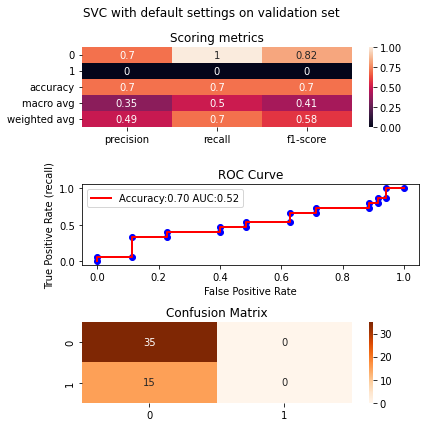
\includegraphics[width=0.5\textwidth]{../project/images/results_default-svc.png}
  \caption{Performance of SVC model with default parameters}
  \label{fig:results_default}
\end{figure}
It is seen that the model scores well in terms of precision, recall and f1-score on class \textit{0}. However, as seen in the confusion matrix this is due to the model classifying all observations to class \textit{0}. This is due to the concerns introduced earlier regarding imbalanced data. As a measure, we balance the weights of each class. This is done by settings the model's \textit{class\_weight} parameter to \textit{balanced}. \textit{class\_weights} can be defined explicitly or have \textit{sklearn} calculate them by the proportions. The validation performance can be seen on Figure \ref{fig:results_default_balanced}.

\begin{figure}[htbp!]
  \centering
  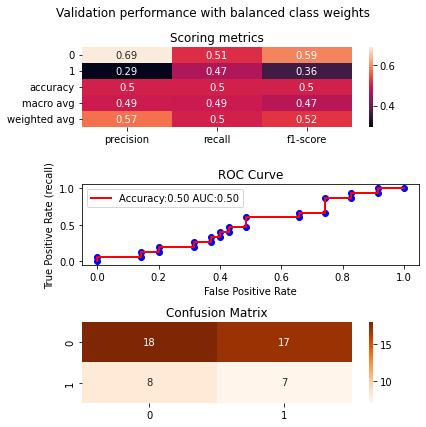
\includegraphics[width=0.5\textwidth]{../project/images/results_default_balanced-svc.png}
  \caption{Performance of SVC model with balanced class weights}
  \label{fig:results_default_balanced}
\end{figure}

The update in class weights clearly makes the model predict more observations to class 1. This leads to better scoring of class 1, but many false positives are introduced as a consequence. To mitigate these, we try to tune other parameters of the model. We do this with \textit{sklearn} \textit{GridSearchCV} implementation. Here we can define a grid of parameters and train models with each combination of the parameters. Additionally, we utilize stratified cross validation with 5 folds. We define a grid with different options for the regularization parameter, C. The performance of the models on each folds can be seen on Figure \ref{fig:results_gridcv_balanced_C}.     

\begin{figure}[htbp!]
  \centering
  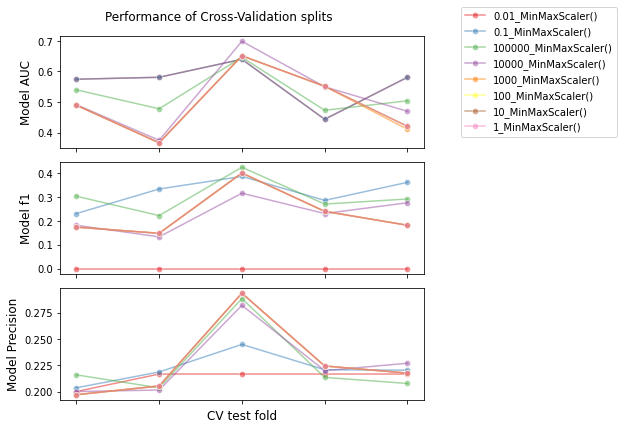
\includegraphics[width=0.5\textwidth]{../project/images/results_gridcv_balanced-C.png}
  \caption{Cross-validation performance of SVC model with different C values}
  \label{fig:results_gridcv_balanced_C}
\end{figure}
There are eight different $C$ values. However, less are showed on the plots. This is due to models performing similarly with nearby values. Looking at the different metrics; AUC, f1, precision, it can be seen that different C values affect the models. Additionally, models performing well at one metric might not succeed according to another metric. The best model is selected according to the average precision metric. The validation performance is evaluated. On figure \ref{fig:results_gridcv_balanced_C_metrics} it shows, that we have less false positives and true positives.   
\begin{figure}[htbp!]
  \centering
  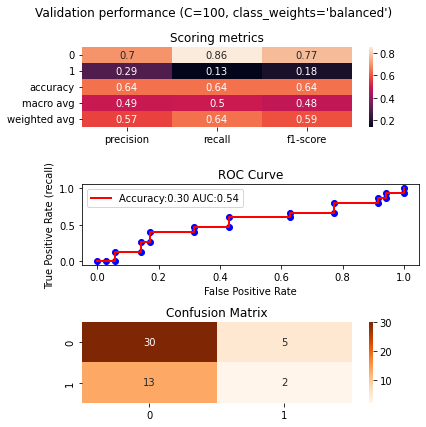
\includegraphics[width=0.5\textwidth]{../project/images/results_gridcv_balanced-C_metrics.png}
  \caption{Performance of best model looking at \textit{C}}
  \label{fig:results_gridcv_balanced_C_metrics}
\end{figure}

There are still many misclassified observations. The next step that we will is feature selection. We will utilize \textit{SelectKBest} with \textit{chi2} as selection method. The selection step is included in the grid search of the best set of parameters. We try with a range of \textit{k} features. The best model according to precision ends up being, \textit{k=21, C=100}. The performance of this model can be seen on Figure \ref{fig:results_gridcv_balanced_C_selKBest}.

\begin{figure}[htbp!]
  \centering
  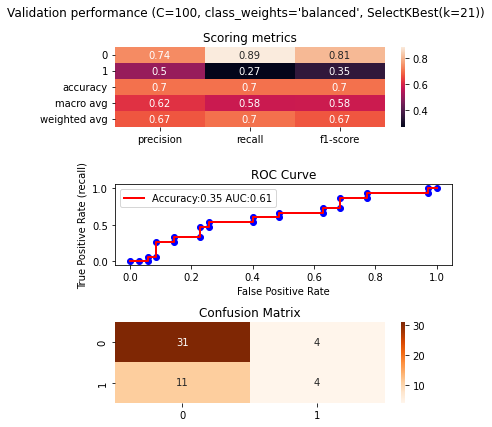
\includegraphics[width=0.5\textwidth]{../project/images/results_gridcv_balanced-C-selectKBest.png}
  \caption{Performance of best model looking at \textit{C} and SelectKBest}
  \label{fig:results_gridcv_balanced_C_selKBest}
\end{figure}

The model seems to identify less false positives while classifying more true positives. Hence, selecting 21 features seems to be positive for the model. Next we will try different kernels of the SVC model. It showed that the default kernel that was utilized already, Radial Basis Functions, is the best performer according to precision.  

\subsection{Kaggle Submission}
The final model is then used to predict labels on the unlabeled test data. The predictions are then submitted to kaggle and evaluated. The result was a score of $0.70666$. This score is low compared to others in the competition. The low score can have various causes, such as:
\begin{itemize}
  \item The model is not well tuned
  \item The model is overfitted on the training data
  \item The data is not preprocessed sufficient
  \item SVM is not the right classifier
\end{itemize}
During the tuning of the model a low range of values was used in the grid search of the optimal parameters. This was due to the necessity of being able to      train the model on a workstation in tolerable time. It would be optimal to try a larger range of values and thus more combinations. 

It is possible that the modes is being overfitted. Meaning the model are learning the wrong concepts from random fluctuations in the training data, that are not present in the test data. Tuning the regularization parameter of SVM and feature selection are both measures against overfitting. However, these might not be sufficient. 

The data might not be sufficiently preprocessed before being used by the model. Data cleaning was performed in terms of filling missing values, scaling was done by transforming the data in a specified range and feature selection was tried. Having additional processing power would allow to test other combinations of scaling and dimensionality reduction techniques. Additionally, it would be interesting to perform some outlier detection. It might be possible that there is some noisy data in the training data. This would also help to avoid overfitting.

Lastly, it might be the case that SVM is not the right model for the problem. SVMs are in general versatile with the use of various kernels. However, as seen in the results of the paper it showed, that even with non linear kernels it was not able to create the right seperating hyperplane. 






\section{Conclusion}
This paper succeeded in developing an AI prediction model to determine if a patient belongs in a specific risk group regarding knee osteoarthritis. Given data was preprocessed by filling missing values, normalizing and feature selection. Different versions of the SVM classifier was evaluated. Resulting in the optimal version having proportionality balanced class weights, a non-linear kernel and utilizing 21 of the original 23 features of the dataset. The performance of the resulting model was underwhelming in terms of precision. The source of the low performance is not clear. However, it might be caused by; model tuning, overfitting, data preprocessing or model selection. 

For future work it would be interesting to look into aquiring more processing power to try out more versions of the model and different data preprocessing steps. This could include a larger range of values of the model's parameters, different scaling techniques and other techniques to fill out missing values in the data. Outlier detection could be used to identify potential noisy data. Additionally, other models than SVM should be investigated.              

\unfinished{Write Conclusion}

\unfinished{Other model}

\unfinished{conclude in regards to clinical setting}

\printbibliography[title={References}]

\end{document}